\documentclass{article}
\usepackage[utf8]{inputenc}
\usepackage{lstautogobble}
\usepackage[export]{adjustbox}
\usepackage{graphicx}
\usepackage{changepage}
\usepackage{listings}
\usepackage{amsthm}
\usepackage{subcaption}
\usepackage{amssymb}
\usepackage{titlesec}
\usepackage{hyperref}
\usepackage{lscape}

%Command to change name of table of contents
\renewcommand*\contentsname{Table of Contents}

%Command to start sections on new pages
\newcommand{\sectionbreak}{\clearpage}

%Create a new "Unlabeled section" that will be added to toc but not printed
\newcommand{\unlabeledsection}[1]{%
 \clearpage
  \par\refstepcounter{section}% Increase section counter
  \sectionmark{#1}% Add section mark (header)
  \addcontentsline{toc}{section}{\protect\numberline{\thesection}#1}% Add section to ToC
  }
  
\emergencystretch=1em

\title{OpenUAS:\\Fifth Semester Progress Report }
\author{ }
\begin{document}


%%TITLE PAGE%%
\maketitle

\newpage

%%TEAM PAGE%%
\begin{center}
\Large \textbf{The OpenUAS Team}

\vspace{1cm}

\large{
Hazel Ambort\footnote[1]{ISU Department of Materials Science and Engineering}\\ John Botsford\footnote[2]{ISU Department of Aerospace Engineering}\\ William Burken\footnote[3]{ISU Department of Mechanical Engineering}\\ Ellie Diersen\footnotemark[2]\\ John Edgren\footnotemark[2]\\ Abigail Gries\footnotemark[2]\\ Madison Harrington\footnotemark[1]\\ Nick Hendrickson\footnotemark[2]\\ Chris Johannsen\footnote[4]{ISU Department of Electrical and Computer Engineering}\\ Stephanie Jou\footnotemark[2]\\ John Levandowski\footnotemark[2]\\ Camryn Medendorp\footnotemark[2]\\ Jordan Reese\footnotemark[2]\\  Alex VandeLoo\footnotemark[2] \footnotemark[4]\\
}\par

\end{center}

\newpage

%%TABLE OF CONTENTS%%

\tableofcontents

%%PROJECT OVERVIEW%%
\section{Project Overview}

\subsection{Purpose}
Currently, there are no open-source unmanned aerial systems (UAS) which are fixed-wing and conceptually available to the general public. There are some similar UAS which are available to the public, but they must be purchased and are not open-source. OpenUAS is producing an open-source, commercial off-the-shelf (COTS) UAS that can be used for educational and research purposes, and it will only consist of components available to the general public, including open-source software.\\\\
Dr. Kristin Rozier, assistant professor within Iowa State's Department of Aerospace Engineering, is the PI on the project. One of her main research areas is system health management for autonomous UAS. Therefore, one of the primary goals for this project is to act as a test bed for her research. As the UAS is also intended to be reconfigurable, it is the end goal that the design can be used in additional research areas as well. Finally, the OpenUAS project is intended to be an educational module for advanced high school and college organizations.\\\\

\subsection{Scope}
In order to develop an open-source, COTS UAS for educational and research purposes that is free and available to the general public, a list of objectives, deliverables, and constraints were identified. The following section will provide an overview of these lists.

\subsection{Objectives}
\begin{enumerate}
\item Create an open-source, affordable, COTS UAS for educational and research flights
\item Provide full documentation of the conception, design, and testing of all systems
\item Act as a test bed for Dr. Rozier's system health management experiments
\item Be easily launched and not require a runway for takeoff or landing. 
\item Be piloted by students and hobbyists
\item Be reconfigurable and support additional components
\end{enumerate}

\subsection{Deliverables}
\begin{enumerate}
\item A functioning design and prototype of a UAS
\item Relevant tools for piloting the UAS from the ground
\item Extensive documentation of the design process
\item Extensive documentation of the manufacturing process
\item Extensive documentation on proper use and safety
\end{enumerate}

\subsection{Constraints}
\begin{enumerate}
\item COTS components
\item Affordable components
\item Easily duplicated components (e.g. all 3D printed parts can be reasonably produced by hobbyists)
\item All components should be reasonably safe (e.g. battery)
\end{enumerate}

%%RELATED WORK%%
\section{Related Work}
\noindent Currently, there are very few comparable fixed-wing UAS. The United States uses UAS such as the RQ-14A Dragon Eye and RQ-11B Raven in its military. Although these UAS are similar in size and weight to the OpenUAS team's target design, the technology and capabilities of these systems are much more advanced, and as such, the budget well exceeds the team's overall budget.\\

\noindent The University of Virginia created the Razor, a small fixed-wing UAS for the Department of Defense. This UAS has a flying wing design and utilizes an Android phone as the main processor. The Razor is of similar size, weight, and performance of the team's target design. One main difference in this system is that it is entirely 3D printed. The team plans on utilizing 3D printing, but not to the extent of the Razor design.\\

\noindent The Albatross is a commercial UAV produced by Applied Aeronautics. Although this aircraft is larger than the team's target design, its performance and low-cost are comparable to the team's goals. This UAV is described in more detail later in the paper, as the team purchased and is beginning to study this design. \\


%%STATUS%%
\section{General Information}

\subsection{Status}
In previous semesters, the OpenUAS team focused on lab organization and development, studying current commercial UAVs, and other smaller side projects. One prototype was finalized in the Spring 2019 semester, however, this model never flew. There were several structural issues that prevented a viable and safe flight. Although no flight testing was performed with this design, the team learned many manufacturing do's and don'ts from it. It also served as the starting place for the current semester's UAS design.\\\\
The first few weeks of the Fall 2019 semester were spent changing design features from the previous model. The wing and tail were the most changed sections of the design, but the fuselage shape was also improved. Computational fluid dynamics (CFD) was performed on the new design before the manufacturing process began mid-semester. Electrical system work was performed in tandem with the airframe design and construction. The last few weeks of the semester were used to flight test the UAS. See Section 5 below for an in-depth overview of the team's work this semester. \\\\

\subsection{Team Organization}
The flowchart on the next page shows the organizational structure of the OpenUAS team. New members joined the team this semester. Many team members are graduating this school year, so it was necessary to fill these positions on the team. Although most new members are not fully apart of the team until the Spring 2020 semester, they attended sub-team and project meetings and shadowed the work of others in the lab. By shadowing the work of the full-time members, the new members will be able to step up and fill the shoes of the graduating students by the end of the Spring 2020 semester. 
\newpage
\begin{landscape}

\begin{figure}[!h]
\begin{center}
	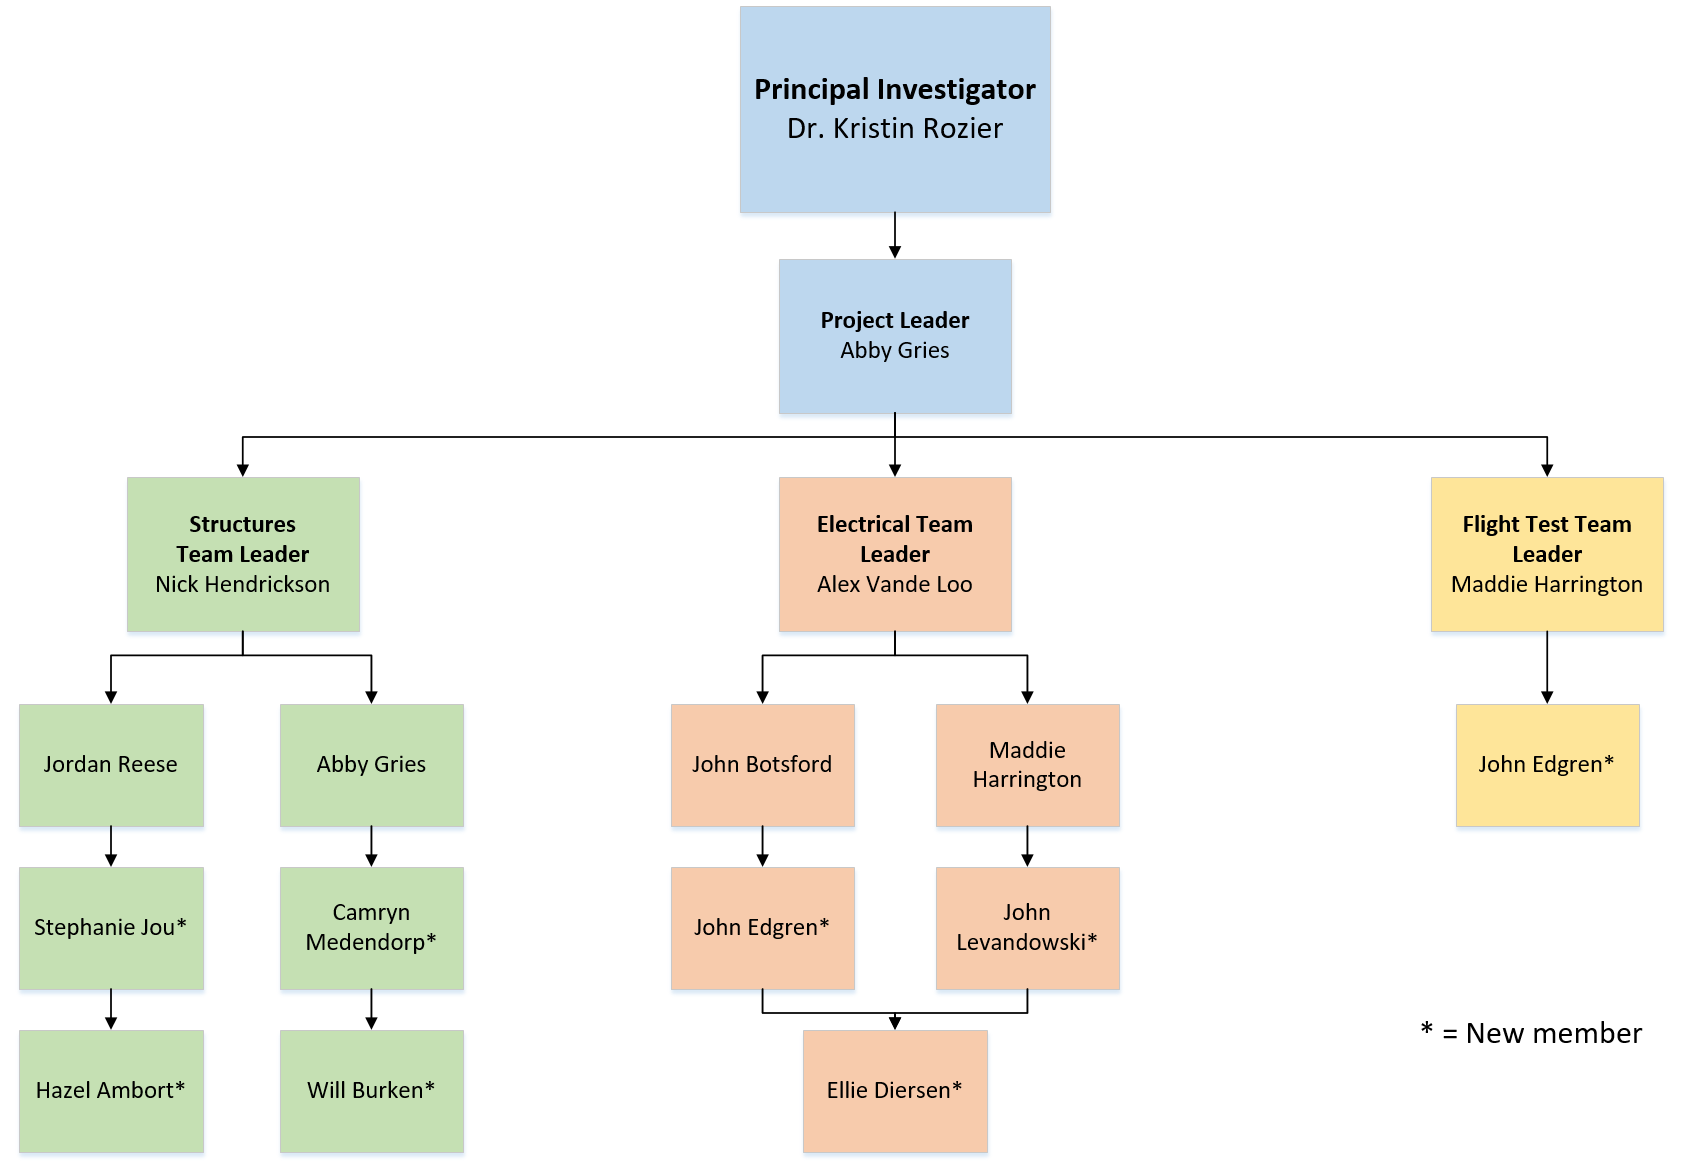
\includegraphics[scale=0.75]{TeamOrganization_Fall2019.png}
	\caption{Fall 2019 Team Organization}
	\label{Figure 1:}
\end{center}
\end{figure}

\end{landscape}

\subsection{Documentation}

Varying forms of documentation were developed to assist with tracking the vision, objectives, high-level project plan, and weekly progress and goals. The documentation is intended to not only support the systems engineering aspect of the project, but also serve an educational purpose by assisting future users who would like insight into what efforts and decisions were made to bring OpenUAS from a concept to a reality. Additionally, everyone on the team keeps their own weekly and semester progress documentation to maintain goals and the vision for every subgroup within the OpenUAS team. 

\begin{enumerate}
\item \textbf{Project Charter}\\ This one-page document was created at the conception of the project and is intended to help provide a broad overview of the project. The Project Charter lays out the scope and purpose of the project. Additionally, the project objectives, deliverables, and constraints that were mentioned earlier in this paper come from the Project Charter. 
\item \textbf{Team Organization}\\ This flowchart shows the organizational structure of the OpenUAS team. The overall team is broken down into three sub-teams: electrical, structures, and flight test. These sub-teams have team leaders and members. The overall project has a project leader. This will change each semester as students join or leave the team. 
\item \textbf{Weekly Meeting Agenda}\\Each week before the team meeting, team leaders update the Weekly Meeting Agenda. This document details the progress made for the week and the goals for the next week. Additionally, team leaders can request assistance through this document and the agenda for the meeting is set by the project leader. Attendance for each meeting is also taken in this document. 
\item \textbf{Requirements}\\ The requirements document is an extensive, volatile artifact that has been developed since the beginning of the project. Originally, our primary requirements were high-level and directly traceable to the overall project goals. Now, as we begin to make decisions about what our design will look like, the requirements have evolved to become more detailed. For the sake of making requirements easier to read and understand, we chose to use the EARS \cite{Terzakis2013} requirements syntax. These requirements will be updated again in the Spring 2020 semester as the next design iteration begins. 
\end{enumerate}

\subsection{Lab Set-Up \& Organization}
\noindent The lab originally started out with no equipment or tools available for our project. Throughout the last school year, orders had been placed for tools and other items needed in order to ensure a work space that has all tools needed for successful progression of this project. This last semester has built off what was completed before, adding new equipment, rearranging tables and desks to provide more surface area in the lab for various projects, and adding more tool locations for easier access to common tools.  Because we are working within a large organization, special documentation and communication must be done in order to acquire the parts needed for the lab. This includes confirmation of successful retrieval of parts and checking if damage was done to them. If damage is found, proceeding with the proper return process and notifications so everyone knows how parts are moving about. If an item is not the item we purchased (e.g. a different sized cartridge for a label printer) we send it back to the individual keeping track of our orders and have them re-order the right equipment. The final goal is to have a lab outfitted in such a way that it can complete any of the tasks designed for the project with exceptions to precision machining and other similar processes.\\


\subsubsection{3D Printer - LulzBot Taz 6}
The LulzBot Taz 6 3D printer was used again this semester to print various components of the OpenUAS model. However, it was not used as extensively as previous semesters as the new structure of the airframe was almost entirely foam and carbon fiber. The two main 3D printed components were the attachments for the wing to fuselage and the plates to hold the components within the fuselage. There were not any issues with printing these components, although in the future, these parts will likely be redesigned or possibly not even used. Specifically, the wing attachments held up well during the testing, but overall, the removable wing design did not work well. Therefore, it is likely that in the future, a more permanent wing design will be created, and the 3D printed wing attachments will become obsolete.\\\\
As discovered in previous semesters, there are some software/firmware issues with the LulzBot Taz 6. The printer and CURA Lulzbot software should still be updated regularly to prevent these issues. It will also be essential to continue to take care of the printer through updates, bed maintenance, and part replacement to keep the printer in the best shape possible. 

%%INSPIRATION: THE ALBATROSS%%
\section{Primary Inspiration: The Albatross UAV}
\noindent The Albatross UAV is a commercial product of Applied Aeronautics. The team purchased this model in the fall of 2017 to study the documentation, the ease of construction, and the flight characteristics of this model. The Albatross UAV has a wingspan of approximately 9.8 feet and is advertised to carry over 4.4 kg of payload over 4 hours. The Albatross is capable of a maximum 90 MPH speed and a cruise of 40 MPH. This UAV has so far been extremely beneficial in the lessons learned from purchasing, documentation, and the construction of UAS in general. 

\subsection{Construction and Progress}
The Albatross was constructed by the end of December in 2018 but has not been flown. The Albatross construction was conducted over two semesters for the OpenUAS team due to severe lack of documentation from the supplier, Applied Aeronautics. From the construction process, the OpenUAS team learned quite a lot from setting up servo connections, the internal organization, drilling into certain components, and in how to better document build processes for future designs. 


\subsection{Looking forward}

While no progress has been made this semester on the Albatross, the team does plan to fly it in the future. This will be useful in testing things like flight modes, gathering flight data, and providing insight into further advancements that can be made for the OpenUAS design. This next semester, in coordination with continuing to fly the OpenUAS models, the OpenUAS team hopes to maintain the Albatross as a flight ready vehicle for any flight-testing needs. 

%%SYSTEM ARCHITECTURE AND PROGRESS%%
\section{OpenUAS System Architecture \& Progress}
This semester the OpenUAS team split into three sub-teams: electrical, structures, and flight test. The structures team was primarily responsible for the airframe design, simulations and calculations (including CFD, center of gravity, stability, etc.), and manufacturing process. The electrical team worked on the hardware, wiring, and software. The flight test team created preflight procedures, ground tests, and the flight tests for the UAS. The following sections describe in detail the work performed by each sub-team this semester. UAS1 refers to the UAS built this semester.  

\subsection{Structures Team}
This section will discuss the design process and decisions made with respect to the OpenUAS prototype that was built this semester.

\subsubsection{Design}
The first step in the design process for the UAS1 was to do research on existing UAS designs. In addition, the UAS1 was designed based on updated versions of previous iterations knowing what design aspects worked and did not work. Once decided on a general design for the craft, SolidWorks was used to generate a 3D model. This helped in the visualization of the design, integration of parts, 3D printing parts, and computer simulations.\\\\
The parabolic shape of the fuselage was chosen to maximize space inside for the electronic systems as well as to minimize the profile drag. The fuselage was designed to hold two boards where the electronic systems can easily be integrated. One of the boards sits on the bottom half of the fuselage while the other board resides in the top half of the fuselage. The board in the upper half of the fuselage is attached by standoffs.\\\\
The airfoil design chosen was the Clark-Y airfoil. The driving factor for choosing this airfoil was the moderate amount of camber. For the UAS1, it was necessary to generate enough lift without creating a large coefficient of moment. From here, the structures team referenced several textbooks and generated spreadsheets to size the wings. Generalized equations were used in this process to predict the amount of lift that would be generated by the wing based on the size. Due to choosing a large chord length for the airfoil, the wing is tapered to decrease the amount of induced drag at the wing tips.\\\\
Finally, the empennage of the UAS1 was designed based off previous iterations of the tail. The team decided to reuse the carbon fiber tube from the previous iteration to attach the tail cone to the fuselage. The tail cone was redesigned to be slightly more aerodynamic and for easier manufacturability. The structures team decided on using a symmetric airfoil for the horizontal stabilizers and the rudder. Again, referencing textbooks, the team sized the horizontal stabilizers based on the size of the wings. Using static stability equations, the team sized the horizontal stabilizers to cancel out the moment generated by the lift from the wings.\\\\


\subsubsection{Computer Simulations}

Once the initial design of the UAS1 was completed and a SolidWorks model was generated, computational fluid dynamic (CFD) simulations were run on the model to determine the aerodynamic characteristics. This process was done in a program called Star CCM+. Once the CFD simulation was performed on the initial design of the UAS1, the team determined the preliminary aerodynamic characteristics. From here, four different performance curves were derived: Cl vs. AoA, Cd vs. Aoa, Cm vs. Aoa, and L/D vs. AoA. It is important to see a negative slope on the Cm vs. AoA curve in the preliminary design of the aircraft. The next step in this process was to determine if the amount of lift generated at a zero angle of attack was sufficient for takeoff. The design needed some adjusting to meet the optimal performance. After each adjustment to the model, a CFD simulation was ran to derive the new performance characteristics. In the case of the UAS1, the angle of incidence of the wings was adjusted to a 3-degree angle of attack at zero pitch. When the aircraft generates a higher lift force compared to its weight and the Cm vs. AoA is a negative slope with a point at (0,0), the design is optimized.

\subsubsection{Manufacturing}

Finally, once the design was finalized the next step was to manufacture the UAS1. At the beginning of the manufacturing process, the team held a meeting to converse the different materials and methods we wanted to use. For the UAS1, we determined to make the fuselage, wings, tail cone, and horizontal/vertical stabilizers out of carbon fiber. First, the team created molds of the structure out of foam to perform a layup on. Next, using the composites lab in Howe Hall, the team did several layups using carbon fiber to create the shell of the UAS1. Finally, all parts were integrated together to create the final product of the UAS1. 

\subsubsection{Launch System}

The launch system of the UAS prototype 1 is a hand launch. With the motor at full throttle, one team member launches the vehicle by hand to establish a fast enough velocity for takeoff. \\\\
The  hand launch failed during the first flight test of the UAS1. The hand launch succeeded on the second flight attempt for UAS1, but a gust of wind caused the aircraft to crash shortly after takeoff. \\\\
Looking forward, the OpenUAS team plans to investigate other launch systems such as a catapult launch and a regular takeoff with landing gear.

\subsection{Electrical Team}

\subsubsection{Software}
The OpenUAS software team created a model for flying the UAS1 that includes the use of flaperons, elevator, and ailerons. The Pixhawk was calibrated and set up in a manner that is compatible with the electrical system (iron bird) for the UAS1. The parameters and controls, after testing and reconfiguring, are reliable and function as desired with the drawback of the flaps not acting as ailerons in the flap flight mode. QGroundControl was the main ground station used and the parameters for the Pixhawk were set through this ground station. The model on the Taranis controller needed to be compatible with the parameters set in QGroundControl and a large amount of time was spent doing this.\\\\
Integration of telemetry with the electrical and structures teams was successful; the avionics system functioned well during the first two flight tests. Feedback was gained from these two flight tests and moving forward this information on servo throws and sensitivities will be taken into account for future flight tests. A new software called OpenTX Companion was used to help setup the Taranis model. This allowed the software team to simulate radio control setup so that the full system did not need to be powered up or even working to do radio tests. This helped speed up the time in which it took to come up with a Taranis model after the set back at the beginning of the semester where the team was back logged in ordering a telemetry cable.\\\\  
The flaperons function as two separate flight modes essentially; flaps are initiated by flipping a switch, otherwise the control surfaces are only acting as ailerons. In the future, the software team would like flaps and ailerons to function within one mode, so that aileron control is possible during takeoff and landing. Updates to the ESC will be looked into so that full throw of the throttle stick can be used. Moving forward with a Pixhawk 4 and full peripherals next semester will allow for more data to be acquired from flight tests. It will be important to streamline the electronics system as well as streamline the software running on it. This will be necessary so that when autonomous flight modes are implemented they will be functioning smoothly and efficiently. Additionally, moving forward, it will be useful to have telemetry call outs from the Taranis controller so that the pilot does not need to pay attention to the ground station to get updates on airspeed.\\\\

\subsubsection{Electronics}
The OpenUAS Electronics team worked to integrate the previous iterations of the electrical system (iron bird) to fit the new model of the UAS1. This involved testing and calibrating many of the components, collaborating heavily with the software team to make sure everything was working as intended, and making small adjustments to the iron bird to fit the new model such as choosing the smaller ESC for the motor and creating a servo rail. Another task through the semester was documentation, as many details from previous semesters had been overlooked and needed to be updated or created altogether to streamline future work.\\\\
Integrating the electrical system with the software and structure systems went very smoothly. Some difficulties were wire management and how that plays into space available for components within the fuselage, running the servo connections, and needing to mount some of the components (i.e. GPS) externally to the craft.\\\\
The electrical system worked well in the first flight test, but one possible cause of failure for the flight test was due to motor power. This was adjusted afterwards by calibrating the ESC to operate at a higher speed. After this adjustment, the thrust seemed to be at a comfortable level with the thrust to weight ratio being close to 1. Another problem was ran into during the second test flight because too small of wire was used to connect the battery to the rest of the system. With the ESC operating at a higher speed, more power was drawn from the battery. This ended up overheating and burning out the wire which then needed to be replaced. This was solved by eliminating a chain of adapters used to connect to the battery and instead just a single, larger gage wire was used. For the third flight test, the electrical system seemed to operate as intended.\\\\
Some progress in documentation was made including taking notes on a general electronics document while conducting tests of the system, creating a wiring diagram for the iron bird, and starting to map connections as a start of a Pixhawk test bed.\\\\
In the future, the electrical team is looking to update the iron bird. This would include looking at the components and make sure none of them are over or under rated which could cause extra power draw on the battery or failure for longer flight tests, continuing to update and refine documentation such as the wiring diagram, working with wire management so that the space in the UAS is used better, and updating the Pixhawk used to the latest version as there have been many problems with the current version.

\subsubsection{Propulsion}
In previous semesters, a motor and propeller were selected to use for the UAS. However, it was discovered this semester that the motor that was purchased is a multi-rotor motor. This motor uses very low pitch propellers, and as such, cannot produce the thrust needed at the cruise speed. This issue was not discovered until later in the semester and to avoid delays in flight testing, a temporary motor was selected. The motor that was selected was a Hacker A40-10XL. Various propellers were considered to use with this motor, but finally, 15x8 and 14x7 APC thin electric propellers were chosen. This decision was based on the manufacturer's recommendation for the motor as well as analysis of the propulsion system using MotoCalc, an online software for propulsion analysis. This selection produced approximately 5.5 lbs of thrust at take-off and produced enough thrust to reach the desired cruise conditions.\\\\
More research should be done in the next semester to better optimize the propulsion system. Different motor and propeller combinations should be analyzed to choose the best configuration based on weight, price, thrust, and power. 

\subsection{Flight Test Team}
The Flight Test team this semester produced preflight procedures, ground tests, and flight tests to be utilized for the UAS prototype testing. These were produced in order to establish clear objectives for each test, to ensure that the procedures are documented, and to enable comprehensive debrief information for documentation purposes. In these tests, any of those wanting to build their own UAS will be able to follow these procedures to ensure flight readiness, control surface manipulation, and proper functioning of the UAS in general. These future flight tests are useful in making structural and software modifications to the design to optimize its performance and provide a reliable public design. \\\\
The team's first flight test took place on 5 December 2019. The team prepared for this flight, but unfortunately after hand launching, the UAS plummeted into the ground. Both wings snapped off, and half the propeller broke off. No other clear damage was made. The team learned from this flight test that perhaps a different propeller, stronger motor (or perhaps higher RPM) was needed, and that it may be useful to pitch up on takeoff, though being conscious of stall speed. The test location was at the Cornerstone Church in Ames, and the majority of the UAS team was there. \\\\
Looking forward, the flight test team will continue to make flight test procedures to provide the entire project with a direction, including clear objectives. For more controlled flights, these procedures will provide reliable flight data. These future tests will include more autonomous integration, testing different onboard components such as lights, cameras, and lidar, testing different structural modifications, and provide reliable performance data for the OpenUAS designs. \\\\


%%LESSONS LEARNED%%
\section{Lessons Learned}

\begin{enumerate}
\item Start the semester with clear objectives, a practical timeline, and organized deliverables
\item If you're having a problem in setting up controls and telemetry, there is probably a solution through adjusting parameters in QGroundControl
\item Things will very often not work the way you think they will
\item Don't rush a project to the point that the results are sloppy, because it will be time consuming to have to correct later
\item Staying organized, especially with wiring/internal components, is incredibly important
\item It is beneficial to have an understanding of the inventory in the lab; spare components that may be useful could be hidden away somewhere
\item When soldering items, make sure they are soldered to the correct spots
\item Try to complete work early - if you leave it until later in the week or day it can get forgotten
\item While in the design process, constantly verify ease of manufacturing
\item Detail progress, especially in construction and instances of problem solving; it's easy to forget what exactly happened and helps all the team members
\item Servo connections can be simplified; for the OpenUAS, the team should have more organized pathways for wiring or just keep all wiring in the fuselage and have extended servo connections with long rods
\item Update the Cura LulzBot software continuously
\item Splicing can save time on some parts and take more time on others
\item A copy of a tool we already have is never a bad thing when two people need to work on the same project
\item Wear safety equipment 
\item Double check your work
\item Not everything works a second time
\item A clean lab is easier to work in than a messy one
\item Debugging takes time, and even more patience 
\item Never plug things into a system when it is powered on
\item Be careful when powering things up using an external power supply
\end{enumerate}

%%LIST OF FUTURE TASKS%%
\section{Future Tasks \& Deliverables}
\begin{itemize}
\item Continue to test fly UAS number one
\item Complete OpenUAS design number two
\item Test fly the Albatross UAV
\item Add onboard components to test: LIDAR, lights, cameras
\item Create and test a new launch system
\item Conduct a fully autonomous flight
\item Implement the Pixhawk4 and its peripherals into UAS number two
\item Set telemetry callouts from the Taranis automatically
\end{itemize}


%%REFERENCES%%
\unlabeledsection{References}
\begin{thebibliography}{100}
\bibitem{Terzakis2013} Terzakis, J. (2013). EARS: The Easy Approach to Requirements Syntax. In International Academy, Research, and Industry Association: The Eighth International Multi-Conference on Computing in the Global Information Technology. Retrieved October 11, 2017, from \\\url{https://www.iaria.org/conferences2013/filesICCGI13/ICCGI_2013_Tutorial_Terzakis.pdf}
\end{thebibliography}


\end{document}
